%% Adapted from GaTech CS 7545 Machine Learning Theory given by Prof. Jacob Abernathy Fall 2018. Original latex file: https://github.com/mltheory/CS7545/blob/master/scribe/CS7545scribe_template.tex 



%%%%%PLEASE CONSIDER CORRECTIONS AT PLACES INDICATED%%%%%%%%
\documentclass{article}
%%%%%Packages Used, add more if necessary%%%%
\usepackage{amsmath,amsfonts,amssymb,graphicx,fullpage,float}
\setlength{\topmargin}{-0.6 in}
\setlength{\textheight}{8.5 in}
\setlength{\headsep}{0.75 in}
\usepackage{mdframed}
\usepackage{multicol}
\usepackage{microtype, hyperref}


%%%%% NO NEED TO EDIT THIS PREAMBLE %%%%%%%%
%%% PREAMBLE %%%
\newcounter{lecnum}
\renewcommand{\thepage}{\thelecnum-\arabic{page}}
\renewcommand{\thesection}{\thelecnum.\arabic{section}}
\renewcommand{\theequation}{\thelecnum.\arabic{equation}}
\renewcommand{\thefigure}{\thelecnum.\arabic{figure}}
\renewcommand{\thetable}{\thelecnum.\arabic{table}}
\newcommand{\lecture}[4]{
   \pagestyle{myheadings}
   \thispagestyle{plain}
   \newpage
   \setcounter{lecnum}{#1}
   \setcounter{page}{1}
   \noindent
   \begin{center}
   \framebox{
      \vbox{\vspace{2mm}
      
      \hbox to 6.28in { 
      {\bf ECE 4252/6252 (FunML) Fundamentals of Machine Learning \hfill 2021--2028} }
      
      \vspace{2mm}
      \hbox to 6.28in { 
      {Courses developed by Professor Ghassan AlRegib 
      (\href{https://alregib.ece.gatech.edu/}{alregib.ece.gatech.edu}) 
      \hfill For inquiries: \href{mailto:alregib@gatech.edu}{alregib@gatech.edu}} }
      
      \vspace{3mm}
      \hbox to 6.28in { {\Large \hfill Lecture #1: #2 \hfill} }
      
      \vspace{2mm}
      \hbox to 6.28in { {\it Co-Instructors: #3 \hfill #4} }
      
      \vspace{2mm}}
   }
   \end{center}

   % -------- PEOPLE OUTSIDE BOX --------
   \vspace{2mm}
   \noindent{\bf Contributors:} Dr. Ahmad Mustafa, Dr. Motaz Alfarraj, Dr. Ashraf Alattar, Dr. Chen Zhou

   \vspace{1mm}
   \noindent{\bf Teaching Assistants} with remarkable contributions include: Kuo-Wei Lai, Wuyang Du, Shiva Mahato, Michael Zhou, Ninghan Zhong

   \markboth{Lecture #1: #2}{Lecture #1: #2}

   \vspace{2mm}
\noindent {\bf Disclaimer}: 
{All content of these notes are part of this course at Georgia Tech. Any re-use or distribution is not permitted without pre-approved permission. All these notes belong to, created by, and copyrighted for Ghassan AlRegib and Mohit Prabhushankar, Georgia Tech, 2021--2028.}

\vspace{2mm}
\noindent {\bf License}: 
{These lecture notes are licensed under the 
\href{https://creativecommons.org/licenses/by-nc-sa/4.0/}{Creative Commons Attribution-NonCommercial-ShareAlike 4.0 International License}.}

   \vspace{2mm}
   \noindent {\bf Errata}: 
   {\it Please submit any errata you find using the following form: 
   \href{https://forms.office.com/r/fbg9dMWPgY}{Errata Form for FunML Textbook} 
   or visit: \url{https://forms.office.com/r/fbg9dMWPgY}}

   \vspace*{4mm}
}
\renewcommand{\cite}[1]{[#1]}
\def\beginrefs{\begin{list}
        {[\arabic{equation}]}{\usecounter{equation}
         \setlength{\leftmargin}{2.0truecm}\setlength{\labelsep}{0.4truecm}%
         \setlength{\labelwidth}{1.6truecm}}}
\def\endrefs{\end{list}}
\def\bibentry#1{\item[\hbox{[#1]}]}

\newcommand{\challenge}[2]{\noindent \textbf{(Challenge Problem)} \emph{#1}: #2 }

\newcommand{\exercise}[1]{\noindent \textbf{(Exercise)} #1 }

\newcommand{\fig}[3]{
			\vspace{#2}
			\begin{center}
			Figure \thelecnum.#1:~#3
			\end{center}
	}
%%% END_OF_PREAMBLE %%%


	
%%%%You may add more \newtheorem if necessary%%%%%%
\newtheorem{theorem}{Theorem}[lecnum]
\newtheorem{lemma}[theorem]{Lemma}
\newtheorem{proposition}[theorem]{Proposition}
\newtheorem{claim}[theorem]{Claim}
\newtheorem{corollary}[theorem]{Corollary}
\newtheorem{definition}[theorem]{Definition}
\newenvironment{proof}{{\bf Proof:}}{\hfill\rule{2mm}{2mm}}


\newcommand{\dom}{\mathrm{dom}}
\begin{document}

%%%%%CHANGE HERE%%%%%%%
%%%%%\section{title of the section} similarly with the rest \section{} or \subsection{} or \subsubsection{} etc


%%%%%CHANGE HERE%%%%%%%%%
%%%%%\lecture{the ordinal number of the lecture}{lecture title}{Jacob Abernethy}{scriber's name}%%%%%%%%
\lecture{27}{Uncertainty Quantification in Neural Networks}{Ghassan AlRegib and Mohit Prabhushankar}{}

%%%%%CHANGE HERE%%%%%%%
%%%%%\section{title of the section} similarly with the rest \section{} or \subsection{} or \subsubsection{} etc

\section{Lecture Objectives}

In this lecture, we study uncertainty quantification in neural networks, which is a fundamental topic for deploying machine learning systems in real-world environments. While traditional machine learning focuses primarily on prediction accuracy, modern applications increasingly require models to also estimate how confident they are in their predictions. This is especially important in safety-critical systems such as healthcare, autonomous driving, and scientific decision making.

We begin by motivating why uncertainty matters from both human cognition and machine learning perspectives. We then introduce the two fundamental categories of uncertainty: aleatoric uncertainty, which arises from inherent noise in the data, and epistemic uncertainty, which arises from limitations in model knowledge. After establishing these foundations, we study practical methods for estimating uncertainty, including iterative methods such as deep ensembles and Monte Carlo dropout, as well as single-pass uncertainty estimation techniques designed for efficient deployment. Finally, we discuss performance metrics used to evaluate uncertainty estimation methods and how these metrics vary depending on the application.

By the end of this lecture, students should understand:
\begin{itemize}
\item Why uncertainty estimation is necessary for trustworthy machine learning.
\item The conceptual difference between aleatoric and epistemic uncertainty.
\item Practical approaches for estimating uncertainty in deep neural networks.
\item How uncertainty estimation is evaluated in practice.
\end{itemize}


\section{Introduction and Motivation}

Uncertainty is an unavoidable aspect of both human reasoning and machine learning systems. In many real-world situations, decisions must be made with incomplete information, noisy observations, or imperfect models. Understanding how to measure and reason about uncertainty is therefore essential for building reliable intelligent systems.

From a machine learning perspective, uncertainty quantification provides a mechanism for determining when a model should trust its predictions and when it should defer to human intervention or additional data collection. Rather than simply producing predictions, modern machine learning systems increasingly must answer an additional question:

\begin{center}
\textit{How certain is the model about this prediction?}
\end{center}

% \subsection{Human Uncertainty}

% Uncertainty is not unique to machine learning; it is a fundamental characteristic of human decision making. Humans constantly operate under uncertainty due to incomplete knowledge, ambiguous sensory input, and cognitive limitations.

% One well-known example is the viral ``Blue or Gold Dress'' image, where different observers perceive the same image differently. Some viewers perceive the dress as blue and black, while others see white and gold. This example illustrates that uncertainty is not merely computational but is deeply rooted in perception and interpretation. Even when given identical data, different observers may arrive at different conclusions.

% Another example arises in medical diagnosis. Consider the task of interpreting chest X-rays. A trained radiologist may confidently distinguish between pneumonia and healthy lungs, while a non-expert may experience significant uncertainty. In such cases, uncertainty often results from lack of experience or insufficient domain knowledge. The appropriate response in human decision making is typically to seek additional expertise or information.

% These examples highlight an important principle that also applies to machine learning:

% \begin{center}
% \textit{Uncertainty often reflects either ambiguity in the data or limitations in knowledge.}
% \end{center}

\subsection{Human Uncertainty}

Uncertainty is not unique to machine learning; it is also a fundamental aspect of human perception and decision-making. Even when two people observe the same data, they may arrive at different conclusions because perception is influenced by context, prior assumptions, and ambiguity in the observed signal. These sources of uncertainty closely mirror the causes of uncertainty in machine learning systems that we will later formalize in Section~\ref{sec:27.3}.

A well-known example is the viral ``Blue or Gold Dress'' image shown in Fig.~\ref{fig:blue_gold_dress}. Some viewers perceive the dress as blue and black, while others see it as white and gold. This example illustrates that uncertainty is not merely a computational issue. Instead, it is deeply connected to how humans interpret sensory information. The underlying pixels in the image do not change, yet people can still produce conflicting interpretations. This makes the example a useful reminder that ambiguity can exist even before we begin designing machine learning algorithms. Later in Section~\ref{sec:27.4}, we will see that this type of ambiguity closely resembles what is known as \textit{aleatoric uncertainty}, where the uncertainty arises from the data itself rather than the observer.

\begin{figure}[H]
    \centering
    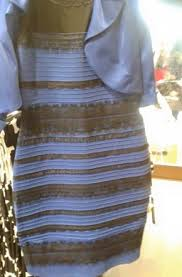
\includegraphics[width=0.28\linewidth]{img/lecture27/blueorgolddress.jpg}
    \caption{Figure 27.1: The viral ``Blue or Gold Dress'' image illustrating how the same visual input can lead to different interpretations due to perceptual ambiguity.}
    \label{fig:blue_gold_dress}
\end{figure}

Another example arises in expert decision-making tasks such as reading chest X-rays, as illustrated in Fig.~\ref{fig:chest_xray_uncertainty}. A trained radiologist may be able to distinguish pneumonia from a healthy chest with relatively high confidence, whereas a non-expert may be much less certain. In this case, the uncertainty comes partly from ambiguity in the image and partly from differences in experience and domain knowledge. This example connects to what we will later define in Section~\ref{sec:27.4} as \textit{epistemic uncertainty}, where uncertainty results from incomplete knowledge rather than inherent data noise. 

\begin{figure}[H]
    \centering
    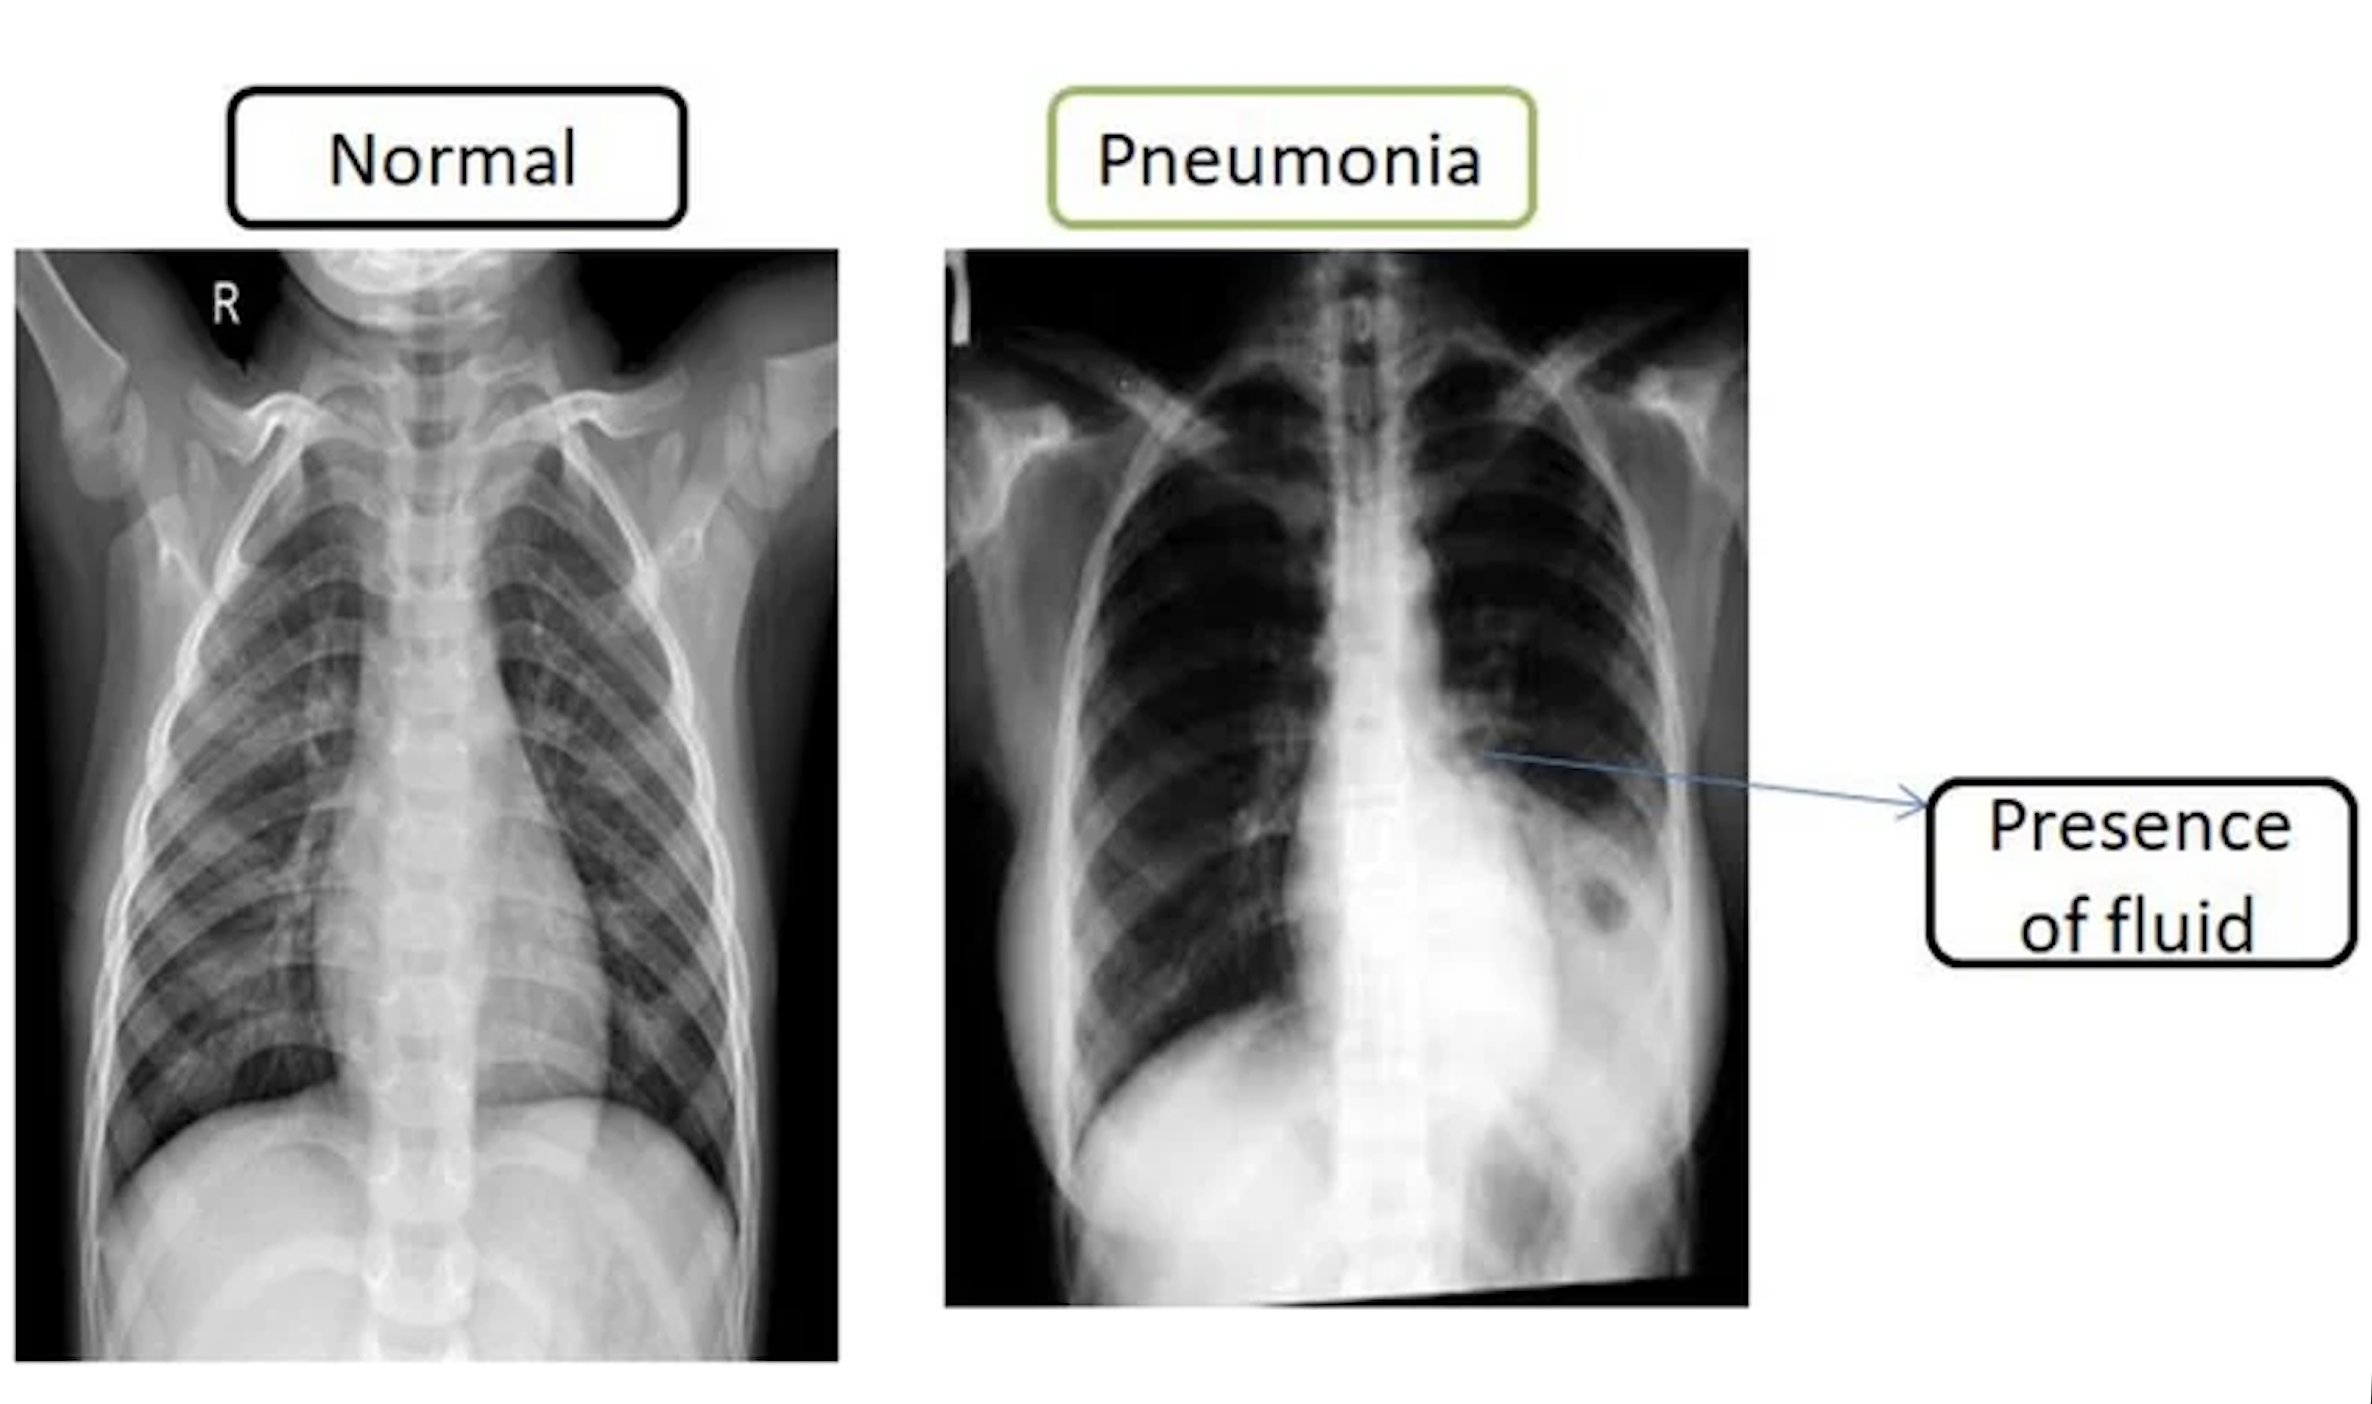
\includegraphics[width=0.65\linewidth]{img/lecture27/Difference-in-Chest-X-Ray-Images-in-Normal-and-Pneumonia.png}
    \caption{Figure 27.2: Comparison between a normal chest X-ray and one showing pneumonia. Medical experts can identify abnormal patterns such as fluid accumulation, while non-experts may not recognize these features. This illustrates epistemic uncertainty arising from differences in knowledge rather than ambiguity in the data itself.}
    \label{fig:chest_xray_uncertainty}
\end{figure}

Together, these examples highlight an important principle that carries over directly to machine learning: uncertainty can arise either because the data itself is ambiguous or because the observer lacks sufficient knowledge to interpret it confidently. These two sources of uncertainty form the foundation for the formal uncertainty taxonomy introduced later in this lecture.

\subsection{Uncertainty Quantification in Neural Networks}

Uncertainty also plays a critical role in machine learning systems. Neural networks typically produce predictions such as classification labels, regression values, or segmentation maps. However, these outputs alone do not communicate how reliable the predictions are.

For example, consider an image segmentation model. The model may assign class labels to each pixel, but without uncertainty estimation we cannot determine which regions of the image were confidently predicted and which were ambiguous. To address this limitation, uncertainty heatmaps can be generated alongside predictions. These maps highlight regions where the model is less confident, allowing practitioners to better interpret model behavior.

Uncertainty quantification is particularly important in safety-critical applications. A well-known example is a fatal autonomous driving accident in which a vehicle failed to detect a truck crossing its path. One contributing factor was that the system did not properly account for its uncertainty regarding the object detection task. If the model had recognized its own uncertainty, it might have triggered additional safety mechanisms.

This motivates a central idea in modern machine learning:

\begin{center}
\textit{Reliable systems must not only make predictions, but also recognize what they do not know.}
\end{center}

\section{Factors that cause uncertainty}
\label{sec:27.3}

Uncertainty in machine learning arises from multiple sources. Understanding these sources is important because different types of uncertainty require different mitigation strategies.

One major source of uncertainty is noise in data acquisition and measurement. Real-world data is rarely perfect. Images may contain blur, sensor noise, lighting variations, weather effects, or occlusions. Similarly, labels may contain errors due to human annotation mistakes. These imperfections introduce variability that cannot always be eliminated, even with better models.

Another source of uncertainty arises from variations among model configurations. Neural networks are typically trained using stochastic optimization methods and random initialization. As a result, two models trained on the same dataset may converge to different solutions and produce different decision boundaries. This variability reflects the model's uncertainty about the correct representation of the data distribution.

A third source of uncertainty comes from unknown or out-of-distribution data. Machine learning models generally assume that test data comes from the same distribution as training data. When this assumption is violated, the model may encounter inputs that lie outside its learned representation. For example, a classifier trained on two classes may encounter a sample belonging to a third unseen class. In such cases, the model may still produce a prediction, but its confidence may be misleading.

These three sources are illustrated in Fig.~\ref{fig:factors_uncertainty}, which shows both variation between model decision boundaries and the impact of unknown samples.

\begin{figure}[H]
    \centering
    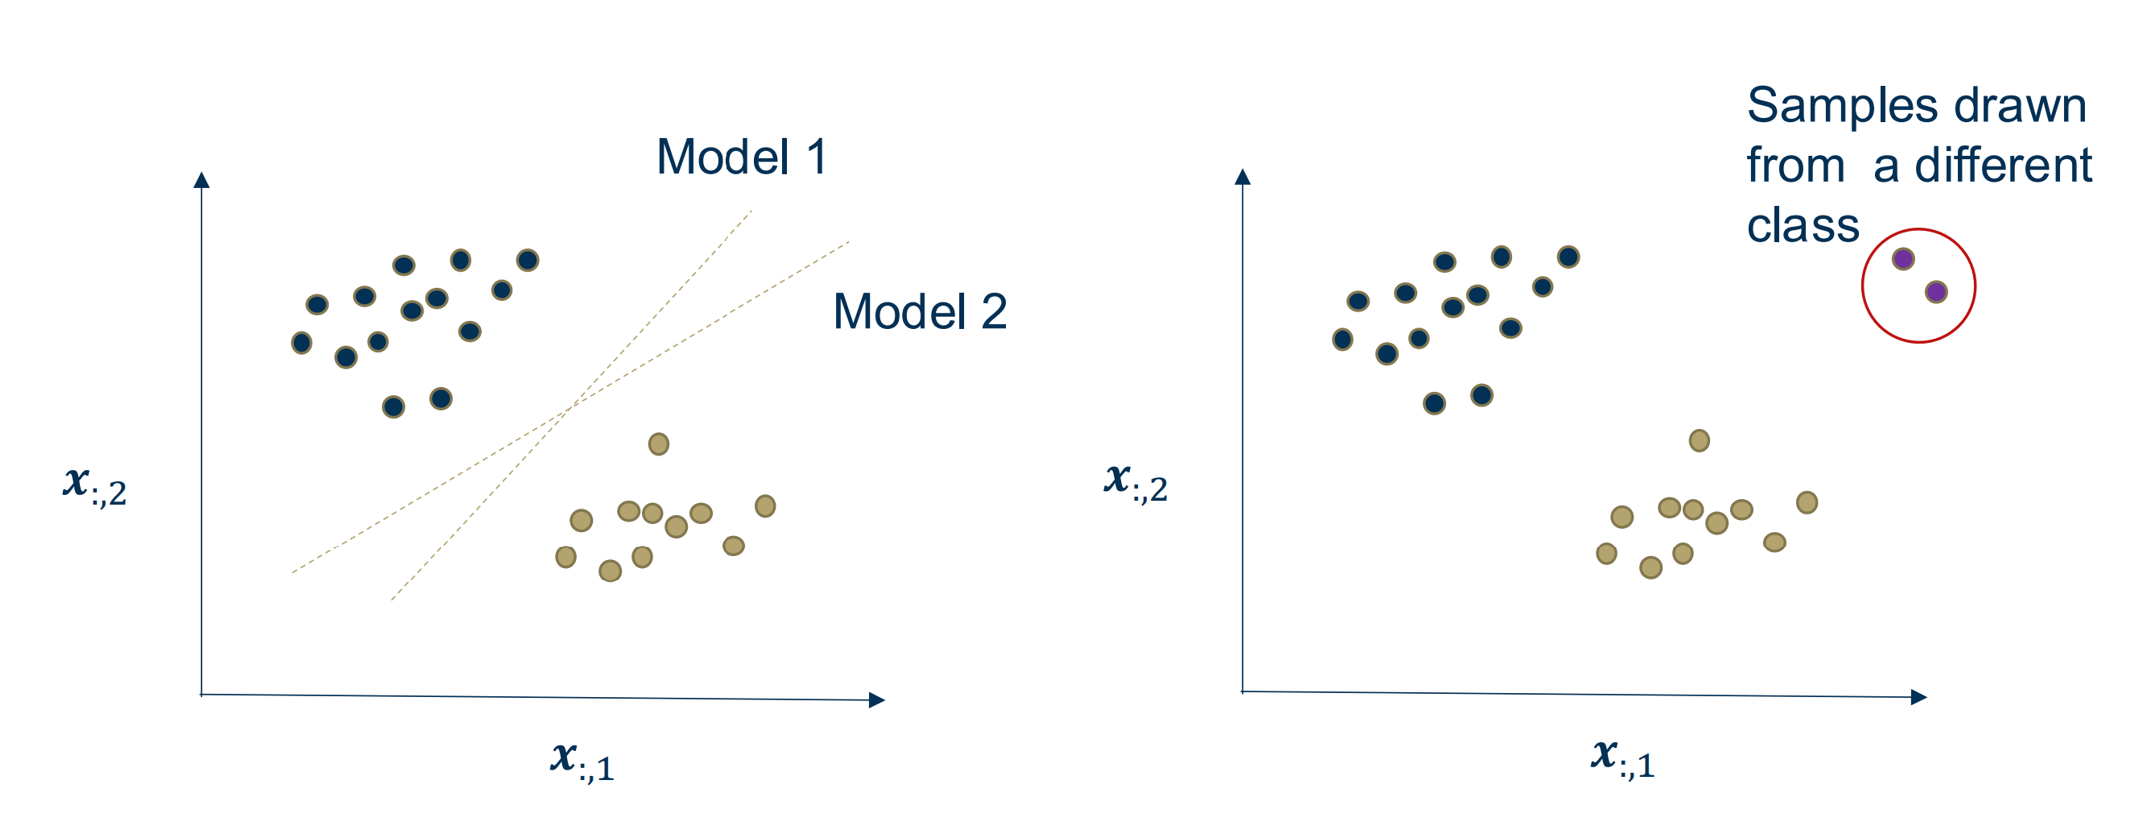
\includegraphics[width=0.8\linewidth]{img/lecture27/factors_uncer.png}
    \caption{Figure 27.3: Factors that Cause Uncertainty. (left) Variations among Model Configurations, (right) Unknown Data}
    \label{fig:factors_uncertainty}
\end{figure}

\section{Two Main Types of Uncertainty}
\label{sec:27.4}

Uncertainty in machine learning is commonly divided into two major categories based on its origin: aleatoric uncertainty and epistemic uncertainty. This distinction is important because it determines whether uncertainty can be reduced.

\subsection{Aleatoric Uncertainty}

Aleatoric uncertainty refers to uncertainty that arises from inherent randomness or noise in the data. This type of uncertainty is often called irreducible uncertainty because it cannot be eliminated even with better models or more training data.

For example, consider predicting the position of a moving object from noisy sensor measurements. Even a perfect model cannot eliminate uncertainty caused by measurement noise. Similarly, images affected by blur or occlusion inherently contain ambiguous information.

Aleatoric uncertainty therefore reflects limitations of the data itself rather than limitations of the model.

\subsection{Epistemic Uncertainty}

Epistemic uncertainty arises from incomplete knowledge of the model. Unlike aleatoric uncertainty, epistemic uncertainty can often be reduced by improving the model, increasing training data, or exploring better architectures.

For example, if a model encounters regions of the input space that were poorly represented during training, it may produce uncertain predictions. Collecting additional data in these regions can reduce epistemic uncertainty.

Thus we can summarize the distinction as follows:

\begin{center}
Aleatoric uncertainty = uncertainty from noisy data

Epistemic uncertainty = uncertainty from limited knowledge
\end{center}


\section{Iterative Uncertainty Estimation}

Epistemic uncertainty refers to uncertainty arising from a model’s lack of knowledge. Unlike aleatoric uncertainty, which is inherent to the data, epistemic uncertainty can often be reduced by improving the model, collecting more data, or exploring the model parameter space more thoroughly. Iterative uncertainty estimation methods provide a practical framework for quantifying this type of uncertainty by repeatedly sampling model predictions under different parameter configurations.

\subsection{Definition}

Iterative uncertainty estimation methods generate multiple predictions for the same input by varying model parameters or network configurations. These multiple predictions are then combined to produce both a final prediction and an uncertainty estimate. Intuitively, this process can be interpreted as exploring different plausible models that could explain the observed data.

More concretely, these methods follow three main steps. First, multiple predictions are generated by varying model parameters through different initializations, stochastic sampling, or architectural perturbations. Second, these predictions are aggregated, typically through averaging, to form a final prediction. Third, the variability among these predictions is used as a measure of uncertainty. If the predictions agree, the model is confident; if they disagree, the model expresses uncertainty.

Next, we examine two representative iterative uncertainty estimation methods: deep ensembles (Sec.~\ref{sec:ensemble}) and Monte Carlo dropout (Sec.~\ref{sec:mc-dropout}).

% Iterative uncertainty methods generate multiple outputs by varying model parameters and then combine them to produce a single uncertainty score. This approach explores the parameter space to better understand the model’s predictions. Key steps in these methods include following:

% \begin{itemize}
%     \item[1.] Iteratively generate multiple model outputs with different parameter constellations.
%     \item[2.] Combine these outputs into a single uncertainty score.
%     \item[3.] This process can be interpreted as exploration of the model's parameter space.
% \end{itemize}

% \noindent Next, we will see two examples of iterative uncertainty methods: Deep ensembles (Sec~\ref{sec:ensemble}) and Monte Carlo dropout (Sec~\ref{sec:mc-dropout}).

\subsection{[Example 1] Deep Ensembles}
\label{sec:ensemble}

\begin{figure}[H]
    \centering
    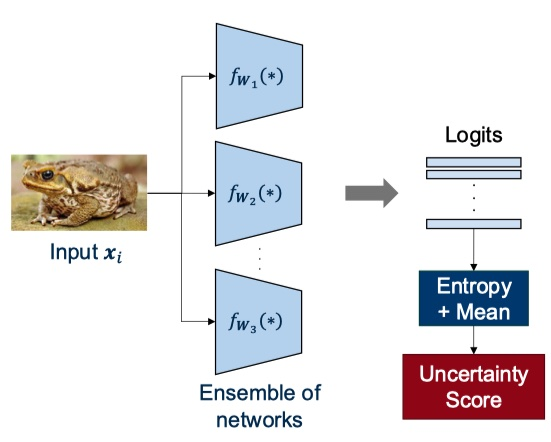
\includegraphics[width=0.5\linewidth]{img/lecture27/deep-ensembles.jpg}
    \caption{Figure 27.4: Deep ensembles generate multiple predictions by training independent neural networks and combining their outputs to estimate uncertainty.}
    \label{fig:deep-ensembles}
\end{figure}

Deep ensembles estimate uncertainty by training multiple neural networks independently and combining their predictions. Each network is initialized differently and may also see slightly different training dynamics due to stochastic optimization. As a result, each network converges to a different local optimum in parameter space. The diversity among these models allows the ensemble to capture epistemic uncertainty.

The final prediction is typically obtained by averaging the outputs of all networks. Uncertainty is then computed using statistics such as the variance of predictions or the entropy of the averaged predictive distribution. If all models agree, uncertainty is low. If predictions differ significantly, uncertainty increases.

Randomness in deep ensembles is typically introduced through different random weight initializations and stochastic training procedures. In some cases, diversity may also be introduced through different training subsets or data augmentations. While this approach provides strong uncertainty estimates, it requires training multiple networks, making it computationally expensive and sometimes impractical for large-scale systems.

From a Bayesian perspective, deep ensembles can be interpreted as approximating sampling from the posterior distribution of model weights. Ideally, we would like to compute the weight posterior:

\[
p(W|x) = \frac{p(x|W)p(W)}{\int p(x|W)p(W)\, dW}
\]

However, the denominator (the marginal likelihood) is typically intractable for deep neural networks. Instead of computing the exact posterior, deep ensembles approximate it by training multiple models that represent plausible solutions. Predictions from these models can then be interpreted as samples from an approximate posterior distribution.

Bayesian Neural Networks (BNNs) provide a more direct attempt to model this posterior by explicitly placing distributions over weights. However, exact inference in BNNs is difficult and often computationally unstable for large models. In practice, deep ensembles often outperform BNNs because they provide a simple and robust approximation without requiring complex posterior inference. One way to interpret this relationship is that BNN predictions resemble noisy samples from a distribution whose mean behavior is captured by deep ensembles.

% Deep ensembles involve training multiple neural networks with different initialization parameters. Each network produces its own prediction, and these predictions are combined to estimate uncertainty. Fig~\ref{fig:deep-ensembles} shows the overall structure of deep ensembles. More details are summarized below.

% \begin{itemize}
%     \item Different initialization parameters lead to diverse network configurations and outputs..
%     \item The final prediction is the average of predictions across all networks.
%     \item Uncertainty scores are computed using entropy and mean of predictions.
%     \item Randomness is introduced in initialization and/or training data. A commonly used method is to initialize weights with different random seeds, while a less common method involves randomly dividing the data into different partitions to train the same network parameters.
%     \item Deep ensembles require training multiple networks, which makes the method computationally expensive and often infeasible for resource-constrained scenarios.
% \end{itemize}


% \noindent\textit{Approximating} deep ensembles involves calculating the posterior distribution of model weights.
% Deep ensembles involve working with the weight posterior, represented as $p(W|x)$, which is defined by below equation.

% $$p(W|x) = \frac{p(x|W)p(W)}{\int p(x|W)p(W) \, dW}$$

% \noindent However, the denominator of this equation is intractable, making direct computation impractical. To overcome this, the posterior is approximated using iterative sampling methods. For a given input $x_i$, multiple samples from the approximate posterior are generated, and the resulting predictions are used to compute entropy and the mean. These metrics are then combined to calculate an uncertainty score, providing insights into the model's confidence in its predictions.

% Previous terminology `posterior' considers the output itself ($p(y|x)$), but weight posterior is in regards to the weight ($p(W|x)$). A related field is Bayesian neural networks (BNN), useful when we have small datasets, since we can get the weight for a neural network by simply sampling from a weight posterior. BNNs are an approximation of deep ensembles, but due to the difficulty of getting the weight posterior they are prone to underperformance in large datasets and models. Overall, BNNs can be interpreted as noisy samples of a distribution with the mean being the deep ensemble.

\subsection{[Example 2] Monte Carlo Dropout (MC-Dropout)}
\label{sec:mc-dropout}

Because deep ensembles require training multiple networks, they can be computationally expensive. Monte Carlo (MC) Dropout provides a more efficient alternative by approximating ensemble behavior using a single network.

In standard dropout, neurons are randomly removed during training to prevent overfitting. During inference, dropout is typically disabled and activations are rescaled to reflect the expected network behavior. MC-dropout instead keeps dropout active during inference. By performing multiple forward passes with different dropout masks, we effectively generate multiple stochastic subnetworks from a single trained model.

These multiple forward passes produce different predictions for the same input. The final prediction is obtained by averaging these outputs:

\[
p(y=c|\boldsymbol{x}) \approx 
\frac{1}{T}\sum_{t=1}^{T}
Softmax(f_{\hat{W}_t}(\boldsymbol{x})),
\quad \hat{W}_t \sim q(W)
\]

Uncertainty is then estimated from the variability of these predictions, often using entropy or variance measures.

The key distinction between standard dropout and MC-dropout is therefore when randomness is applied. Standard dropout introduces randomness only during training and uses deterministic inference. MC-dropout introduces randomness during both training and inference, allowing uncertainty to be estimated through repeated stochastic forward passes.

\begin{figure}[H]
    \centering
    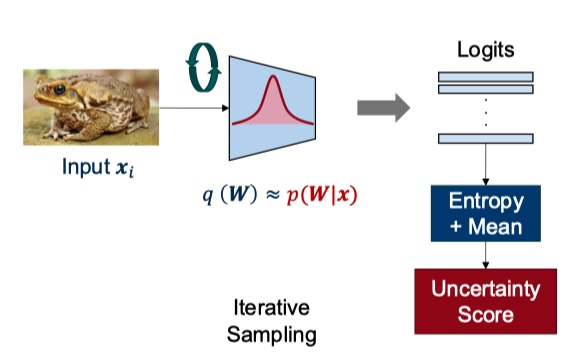
\includegraphics[width=0.5\linewidth]{img/lecture27/MC-dropout.jpg}
    \caption{Figure 27.5: Monte Carlo dropout approximates an ensemble by performing multiple stochastic forward passes using dropout at inference time.}
    \label{fig:mc-dropout}
\end{figure}

\subsection{Summary}

Both deep ensembles and MC-dropout estimate uncertainty by generating multiple predictions and measuring their agreement. Conceptually, both methods approximate sampling from a distribution over plausible models. Deep ensembles achieve this by explicitly training multiple models, while MC-dropout approximates this behavior through stochastic sampling within a single network.

\begin{figure}[H]
    \centering
    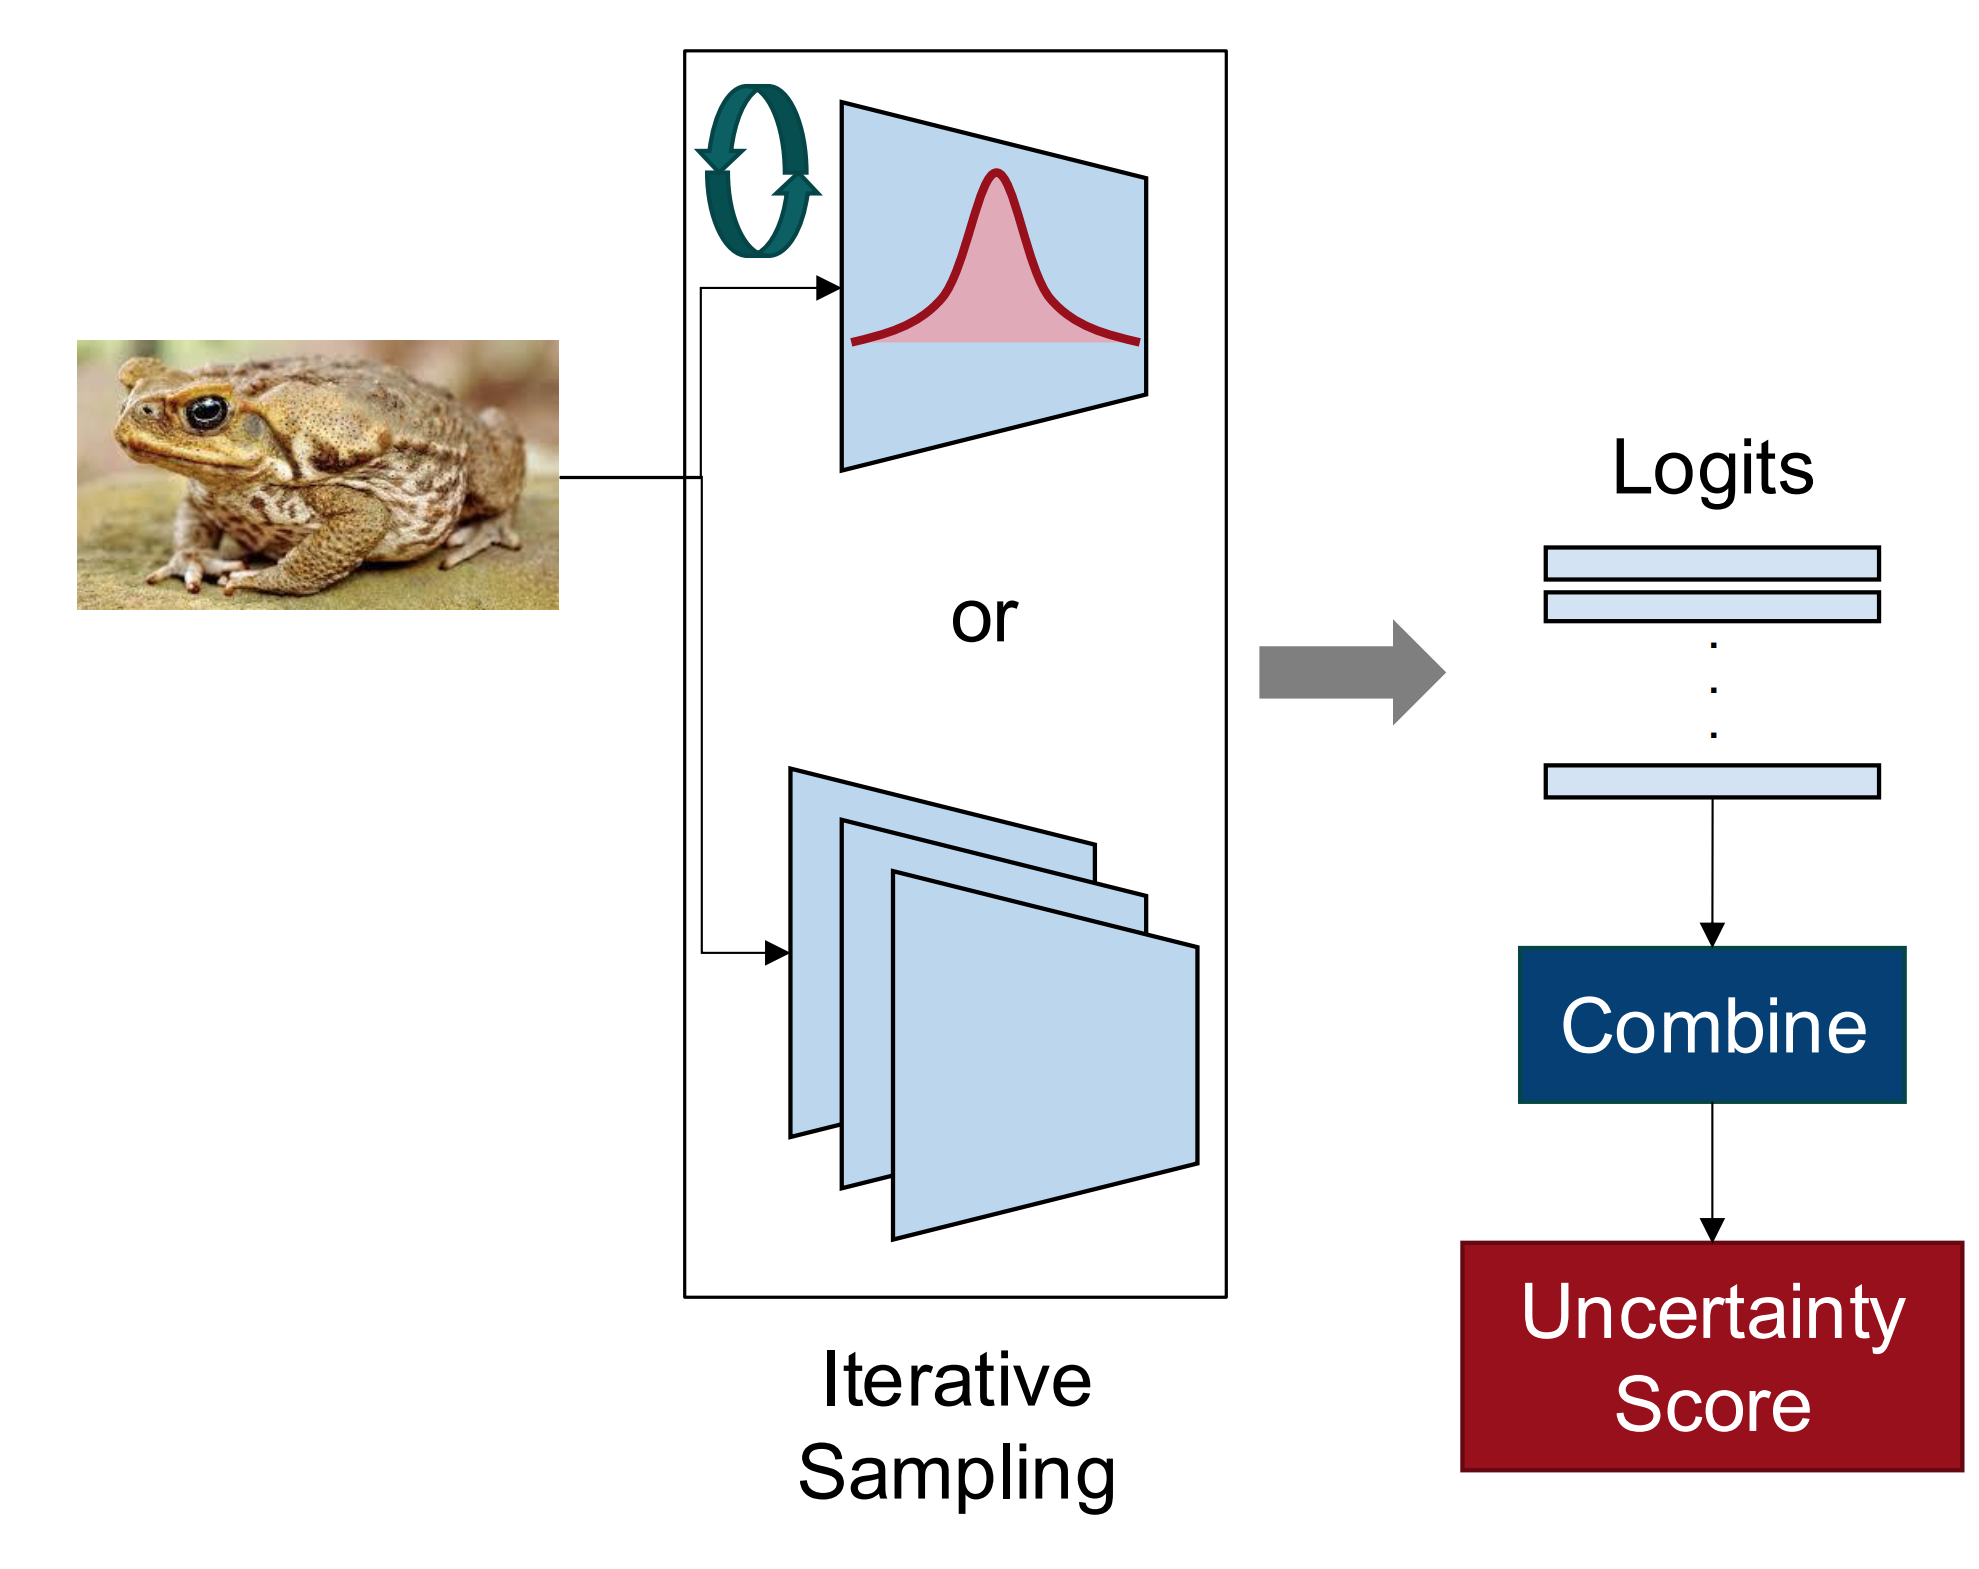
\includegraphics[width=0.5\linewidth]{img/lecture27/iterative_sampling_summary.png}
    \caption{Figure 27.6: Summary of iterative uncertainty estimation methods.}
    \label{fig:iter_summary}
\end{figure}

% To calculate the uncertainty, we can first formulate the total uncertainty as the sum of aleatoric and epistemic uncertainty. It's possible to directly calculate the total and aleatoric (we can quantify aleatoric uncertainty, but can't perform reduction) uncertainty with the equation  shown bellow. 
% $$U_{epistemic} + U_{aleatoric} = U_{total}$$
% $$U_{epistemic} = U_{total} - U_{aleatoric} = H(\frac{1}{T} \Sigma_{t=1}^{T} Softmax(f_{\hat{W_t}} (\boldsymbol{x})) - \frac{1}{T} \Sigma_{t=1}^{T} H(Softmax(f_{\hat{W_t}}(\boldsymbol{x})))$$
% Here, aleatoric uncertainty is the mean of entropy (e.g. Shannon entropy $(plog(p))$) of each logit and total uncertainty is the entropy of the mean of each logit. 

% \begin{figure}[h]
%     \centering
%     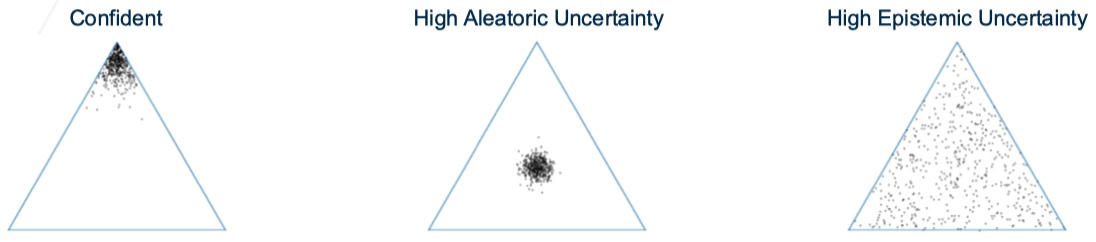
\includegraphics[width=0.8\linewidth]{img/lecture27/uncertainty-summary.jpg}
%     \caption{Visualization between confident, high aleatoric uncertainty, and high epistemic uncertainty.}
%     \label{fig:enter-label}
% \end{figure}
% The visualization of different types of uncertainty in Fig~\ref{fig:enter-label} follows the visualization scheme from Lecture 25 (Active Learning). The triangle vertices indicate three different classification labels, whereas the edges represent the posterior probability of each class. The main difference is that in Fig~\ref{fig:enter-label}, each dot represents different neural network \textit{models} for a \textit{same} data point, rather than different data points from a same model. 
% \begin{itemize}
%     \item When uncertainty is low and the model is \textit{confident}, dots are packed into one vertex. 
%     \item \textit{High aleatoric uncertainty} shows models' indecisiveness among the three labels, leading to similar posterior probability for all classes. In this case, all models agree they don't know a correct answer. Since the uncertainty originates from the data itself, it is impossible to be improved, even with more powerful computational resources or with better models.
%     \item \textit{High epistemic uncertainty} showcases different models giving different predictions scattered over the space.
    
% \end{itemize}

% \noindent One thing to note is that aleatoric and epistemic uncertainty represent different ideas, so we cannot infer aleatoric from epistemic and vice versa.

To better understand how these methods quantify uncertainty, we can examine how predictive uncertainty is decomposed into its fundamental components. A useful decomposition separates total uncertainty into aleatoric and epistemic components:

\[
U_{total} = U_{epistemic} + U_{aleatoric}
\]

Total uncertainty can be measured as the entropy of the averaged predictive distribution, while aleatoric uncertainty can be measured as the average entropy of individual predictions:

\[
U_{epistemic}
=
H\!\left(
\frac{1}{T}
\sum_{t=1}^{T}
Softmax(f_{\hat{W}_t}(\boldsymbol{x}))
\right)
-
\frac{1}{T}
\sum_{t=1}^{T}
H\!\left(
Softmax(f_{\hat{W}_t}(\boldsymbol{x}))
\right)
\]

Here, aleatoric uncertainty reflects noise inherent in the data, while epistemic uncertainty reflects disagreement among models. Because epistemic uncertainty arises from model knowledge gaps, it can often be reduced through better models or more data.

\begin{figure}[H]
    \centering
    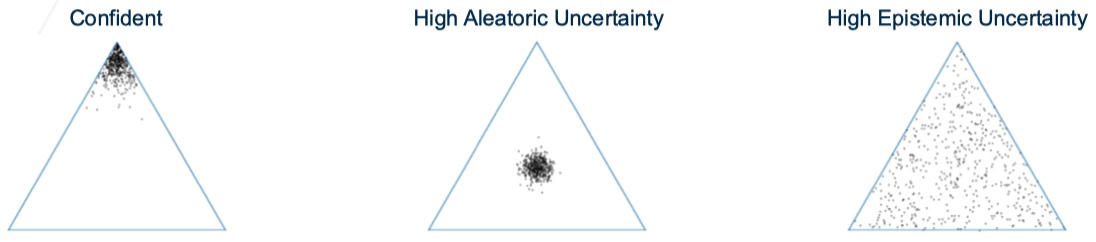
\includegraphics[width=0.8\linewidth]{img/lecture27/uncertainty-summary.jpg}
    \caption{Figure 27.7: Visualization of confident predictions, high aleatoric uncertainty, and high epistemic uncertainty.}
    \label{fig:uncertainty_types}
\end{figure}

Figure~\ref{fig:uncertainty_types} visualizes these uncertainty types using a probability simplex. Each vertex represents a class label, and each point corresponds to a model prediction for the same data point. When predictions cluster near one vertex, the model is confident. High aleatoric uncertainty appears when predictions concentrate near the center, indicating inherent ambiguity in the data. High epistemic uncertainty appears when predictions are scattered, indicating disagreement among models.

Importantly, aleatoric and epistemic uncertainty represent fundamentally different sources of uncertainty. Aleatoric uncertainty cannot be reduced through better modeling, while epistemic uncertainty often can.

The main tradeoffs between these iterative uncertainty estimation methods are summarized in Table~\ref{tab:iter_uncertainty}.

\begin{table}[H]
\centering
\begin{tabular}{lcc}
Method & Cost & Uncertainty Quality \\
\hline
Deep Ensemble & High & Very strong \\
MC Dropout & Medium & Good \\
BNN & Very High & Theoretical
\end{tabular}
\caption{Comparison of iterative uncertainty methods}
\label{tab:iter_uncertainty}
\end{table}

In practice, deep ensembles are preferred when computational resources permit, while MC-dropout provides a practical alternative when efficiency is important.

\subsection{Application: Uncertainty Quantification in Segmentation Applications}

A practical application of uncertainty quantification arises in image segmentation tasks, particularly in safety-critical domains such as medical imaging and autonomous driving. In these settings, knowing \textit{where} a model is uncertain can be just as important as the prediction itself.

Figure~\ref{fig:iterative_application} illustrates an example segmentation result together with corresponding aleatoric and epistemic uncertainty maps. The ground truth and model prediction are shown alongside visualizations of the two uncertainty types.

Consistent with the characteristics of aleatoric uncertainty, the highest aleatoric values typically appear near class boundaries. These regions often contain inherent ambiguity due to noise, limited image resolution, or gradual transitions between classes. Since this uncertainty originates from the data itself, it generally cannot be reduced through improved modeling.

In contrast, epistemic uncertainty tends to appear in localized regions where the model lacks sufficient knowledge. These regions may correspond to rare structures, unusual textures, or examples that are underrepresented in the training data. Unlike aleatoric uncertainty, epistemic uncertainty can often be reduced by collecting more data or improving the model.

This example highlights an important practical benefit of iterative uncertainty estimation methods: they allow practitioners not only to obtain predictions, but also to identify \textit{where} those predictions may be unreliable. Such information is often used in practice to guide data collection, trigger human review, or improve model robustness.

\begin{figure}[H]
    \centering
    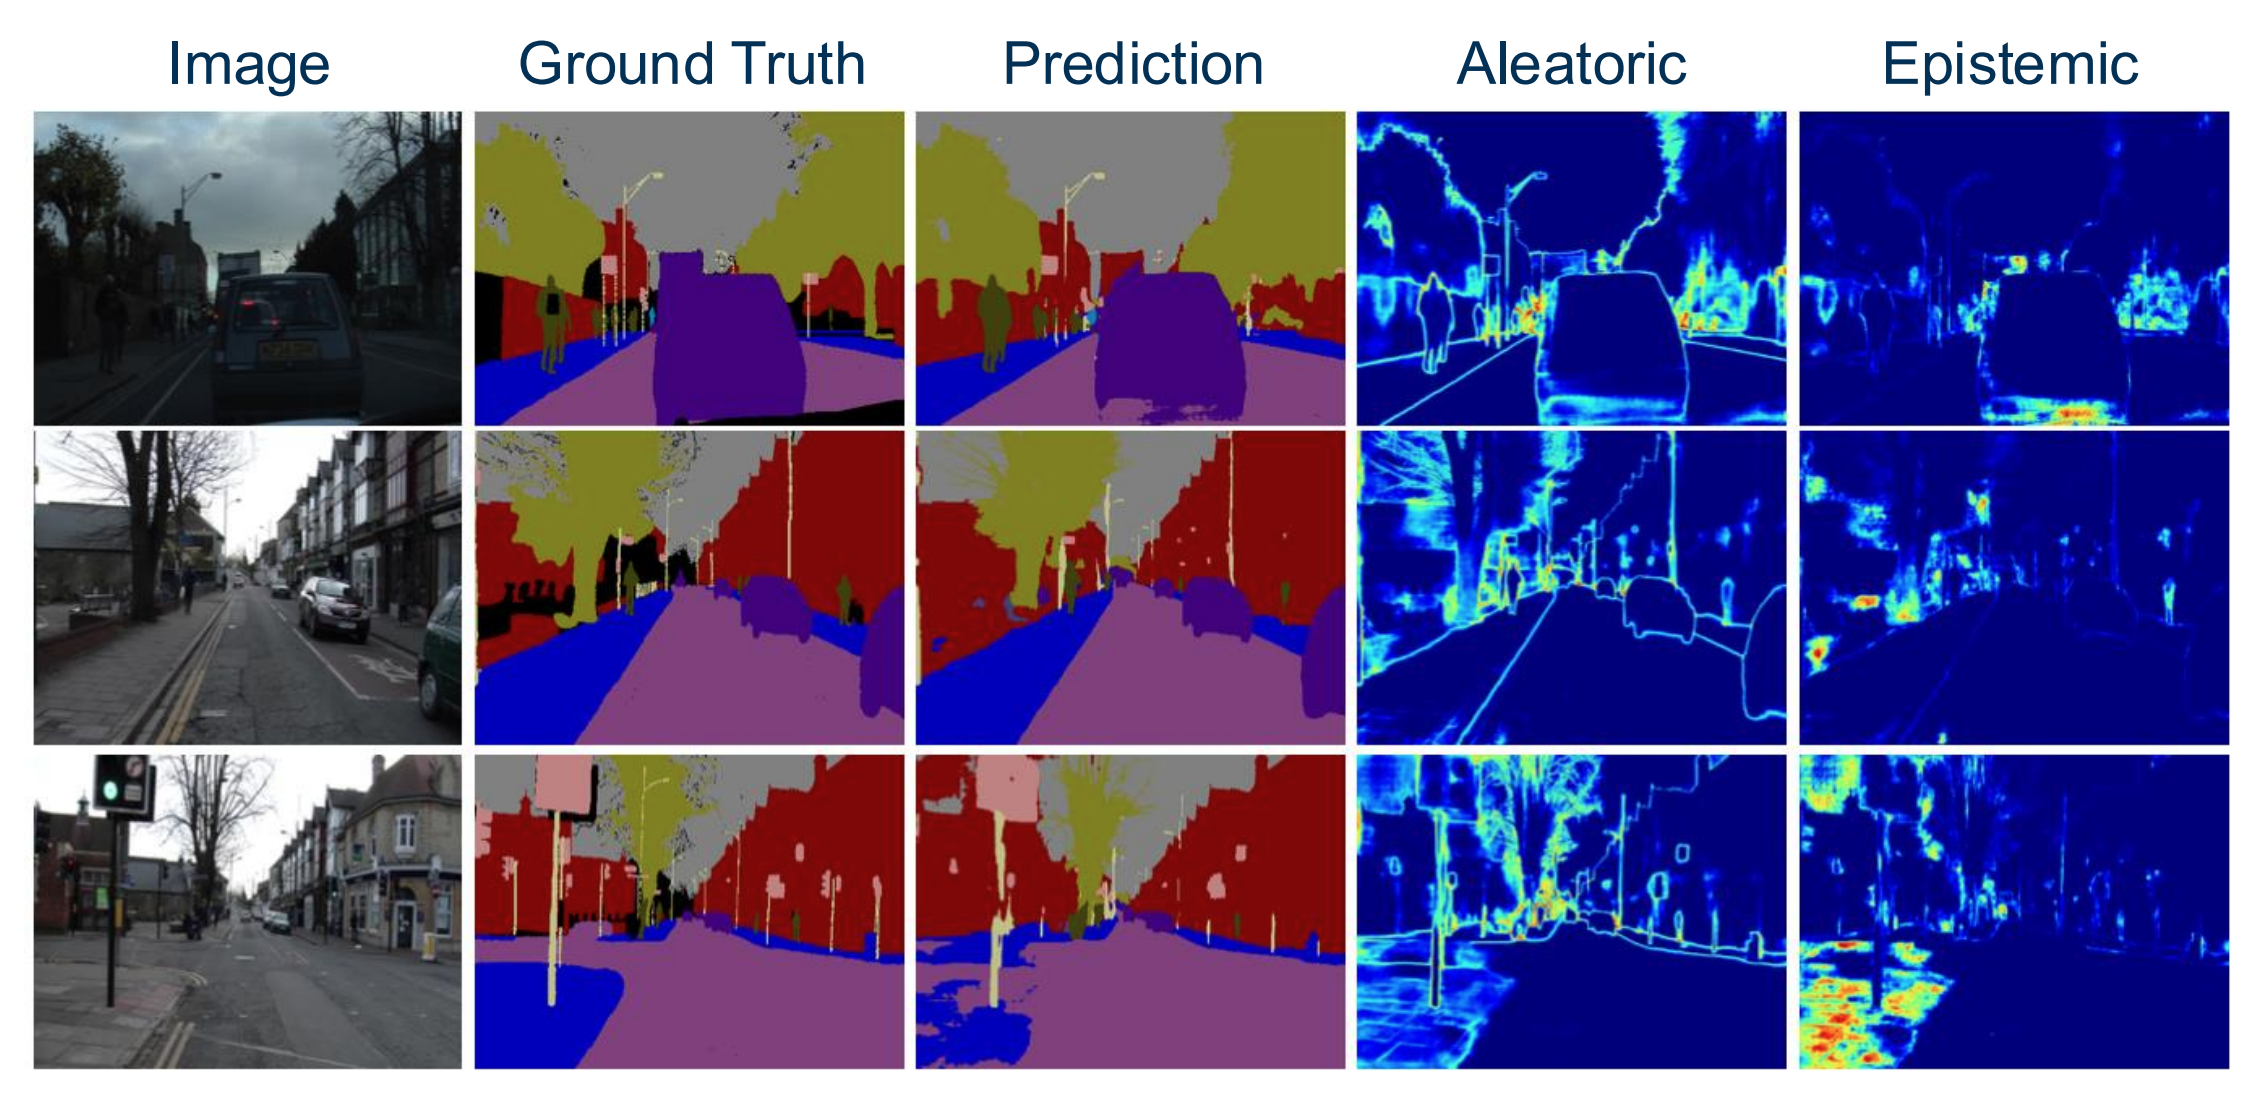
\includegraphics[width=0.8\linewidth]{img/lecture27/uncertainty_application_segmentation.png}
    \caption{Figure 27.8: Uncertainty Quantification in Segmentation Applications}
    \label{fig:iterative_application}
\end{figure}

\section{Single Pass Uncertainty Estimation}

\subsection{Difficulty-based Methods}

Although iterative uncertainty estimation methods such as deep ensembles and MC-dropout provide strong uncertainty estimates, they can be computationally expensive because they require multiple forward passes or multiple trained models. In many real-world applications, such repeated computation may be impractical due to latency constraints or limited computational resources. This motivates the development of \textit{single pass uncertainty estimation} methods, which estimate uncertainty from a single forward pass of a neural network.

Single pass methods typically rely on additional assumptions about the structure of the model or the prediction space in order to approximate uncertainty without repeated sampling. These approaches are closely related to the ideas introduced in Lecture 25 on active learning. In fact, many uncertainty estimation techniques can be interpreted as precursors to active learning methods, since both attempt to identify informative or uncertain samples.

Recall that the goal of active learning is to select the most informative samples for labeling in order to improve model performance with minimal supervision. This is typically achieved through the design of an acquisition function that measures the usefulness of candidate samples. These acquisition strategies generally fall into two categories: difficulty-based methods and diversity-based methods.

Difficulty-based methods prioritize samples that the model finds difficult to classify. These samples typically lie near decision boundaries where prediction confidence is low. By focusing on these uncertain samples, the model can refine its decision boundaries. In contrast, diversity-based methods select representative samples that capture the overall structure of the data distribution, often focusing on central regions of clusters rather than boundary regions.

Single pass uncertainty estimation primarily adopts the difficulty-based philosophy. Instead of performing multiple model evaluations, uncertainty is estimated directly from the predictive distribution produced by a single forward pass. Common measures include entropy, least-confidence scores, and prediction margins. These measures attempt to quantify how uncertain the model is about its prediction based solely on output probabilities.

However, a key limitation of difficulty-based uncertainty scores is their sensitivity to outliers. Models may assign high uncertainty to samples that are far from the training distribution, even when these samples are not informative for improving the model. This can lead to poorly calibrated uncertainty estimates, where uncertainty scores do not accurately reflect prediction reliability.

The general paradigm of single pass uncertainty estimation is illustrated in Fig.~\ref{fig:paradigm_single_pass}. Given a test input $x$, the model produces a latent representation $f_W(x)$ and a corresponding predictive distribution. Uncertainty is then computed from the output distribution rather than from multiple model evaluations.

The main quantities shown in Fig.~\ref{fig:paradigm_single_pass} are:

\begin{itemize}
    \item $\boldsymbol{U^*}(x)$: the estimated uncertainty of test point $x$
    \item $f_W(x)$: the latent feature representation produced by the network
    \item $U(f_W(x))$: uncertainty estimated from the output prediction
\end{itemize}

\begin{figure}[H]
    \centering
    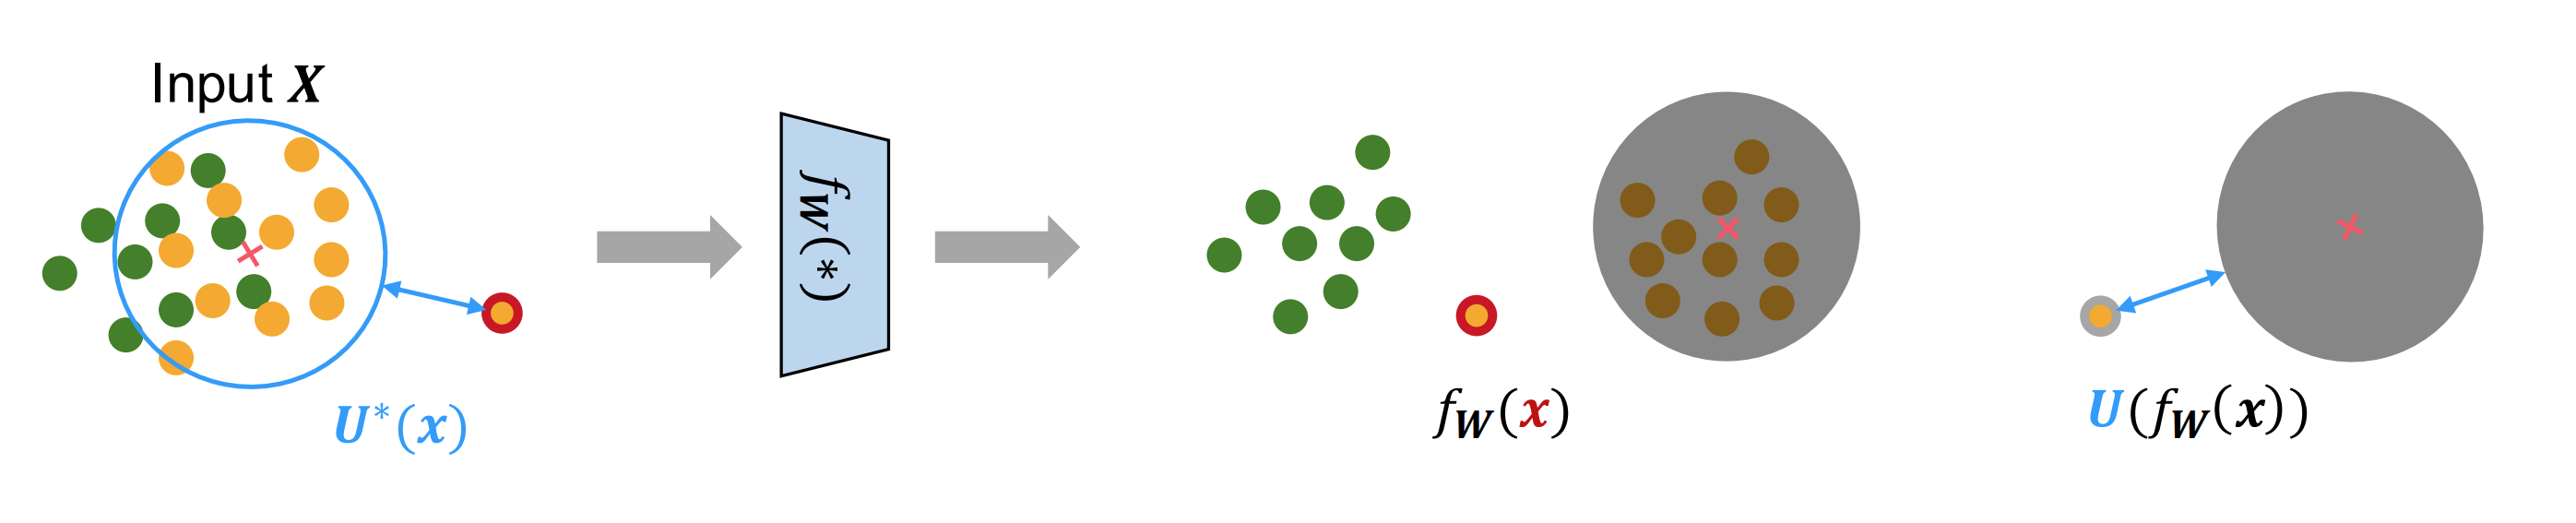
\includegraphics[width=1\linewidth]{img/lecture27/paradigm_of_single_pass.png}
    \caption{Figure 27.9: Typical paradigm of single-pass uncertainty estimation.}
    \label{fig:paradigm_single_pass}
\end{figure}

A common interpretation of this framework is that uncertainty increases as the distance between a test sample and known training representations increases. However, this interpretation introduces an important challenge: uncertainty is typically measured in the latent feature space rather than the original input space.

This mismatch can lead to calibration problems. For example, the highlighted yellow data point in Fig.~\ref{fig:paradigm_single_pass} may be clearly distinguishable in the original input space but may appear ambiguous in the learned feature space due to imperfect feature representations. Without ground truth labels, the model may incorrectly interpret this sample as uncertain even though it is easily classifiable.

This illustrates a key limitation of naive single-pass uncertainty estimation: the quality of uncertainty estimates depends heavily on the quality of the learned feature space.

\subsection{Distance-preservation Methods (Optional)}

To address these limitations, distance-preserving models have been proposed. The main idea behind these methods is to ensure that distances between samples in the input space are meaningfully preserved in the learned feature space. If this property holds, uncertainty estimates based on feature distances become more reliable.

One common approach is to impose a Bi-Lipschitz constraint on the learned representation:

\[
L_1||\boldsymbol{x} - \boldsymbol{x'}||_X 
\leq 
||f_W(x) - f_W(x')||_H 
\leq 
L_2 ||\boldsymbol{x} - \boldsymbol{x'}||_X
\]

This constraint enforces two desirable properties. The lower bound prevents the network from collapsing distinct inputs into identical feature representations, which would destroy useful distance information. The upper bound prevents excessive sensitivity, where small changes in input produce large and unstable changes in feature space.

Together, these constraints promote stable and meaningful representations by balancing sensitivity and smoothness. This helps prevent feature collapse and improves the reliability of uncertainty estimates derived from latent representations.

In practice, distance preservation improves uncertainty calibration because samples that are clearly separable in input space remain separable in feature space. As a result, uncertainty estimates better reflect true model uncertainty rather than artifacts of representation learning.

\section{Performance Metrics}

Evaluating uncertainty estimation is fundamentally more challenging than evaluating standard prediction performance. Unlike classification accuracy or regression error, uncertainty does not have a single universal metric because it is not a prediction itself, but rather a measure of confidence in a prediction. As a result, the choice of evaluation metric often depends on how the uncertainty estimate will be used in practice.

Uncertainty is a general concept that applies equally to both classification and regression problems. Just as classification and regression require different performance metrics, uncertainty estimation also requires task-dependent evaluation criteria. In this sense, evaluating uncertainty is similar to evaluating explainability methods: there is no single best metric, and performance must be assessed based on the intended application.

Uncertainty estimation remains an active research area, and many evaluation approaches continue to be developed. Broadly, existing evaluation strategies can be divided into three categories: per-sample metrics, per-dataset metrics, and application-driven metrics.

\begin{itemize}
    \item \textbf{Per-sample metrics:} evaluate the quality of uncertainty estimates for individual predictions (e.g., Negative Log-Likelihood and Brier score)
    \item \textbf{Per-dataset metrics:} evaluate whether uncertainty correlates with model errors across a dataset (e.g., misprediction detection)
    \item \textbf{Application-based metrics:} evaluate how uncertainty improves downstream tasks such as active learning or open-set recognition
\end{itemize}

\subsection{Per-sample Uncertainty}

Per-sample uncertainty metrics evaluate how well the model's predicted probability distribution reflects the true outcome. These metrics typically require ground-truth labels and therefore are most useful in evaluation settings rather than deployment scenarios.

Two commonly used metrics are Negative Log-Likelihood (NLL) and the Brier score.

Negative Log-Likelihood (NLL) measures how well the predicted probability distribution explains the observed data. For a correct prediction, assigning high probability leads to a low NLL value, while assigning low probability leads to a high NLL value. Therefore, lower NLL values indicate better calibrated predictions and lower predictive uncertainty.

NLL is derived from probabilistic modeling and Bayesian learning, where model quality is measured based on how likely the observed data is under the learned distribution. This metric is widely used in probabilistic regression and classification models and is particularly useful when models output full predictive distributions rather than point estimates.

The Brier score measures the mean squared error between predicted probabilities and the true labels. Unlike NLL, which focuses on likelihood, the Brier score directly measures calibration error by evaluating how close predicted probabilities are to true outcomes. A lower Brier score indicates better calibrated predictions, while a higher score indicates poorer uncertainty estimates.

Intuitively, the Brier score penalizes both incorrect predictions and overconfident predictions. This makes it particularly useful for evaluating probabilistic classifiers.

A key limitation of both NLL and Brier score is that they require ground-truth labels. In many real-world scenarios, such labels may not be immediately available, limiting the usefulness of these metrics for real-time uncertainty evaluation.

\subsection{Per-dataset Uncertainty: Misprediction Detection}

Per-dataset uncertainty metrics evaluate whether uncertainty estimates correlate with model errors across an entire dataset. Instead of evaluating individual predictions, these metrics measure whether uncertain predictions are more likely to be incorrect.

One common approach is misprediction detection, which evaluates whether uncertainty scores can distinguish correct predictions from incorrect ones. This can be measured using ranking-based metrics such as area under the curve (AUC).

An example evaluation procedure using the ImageNet validation dataset (50,000 images) follows these steps:

First, inference is performed on the entire validation dataset to obtain predictions and corresponding uncertainty scores. In the example shown in Fig.~\ref{fig:gradtrust}, GradTrust is compared against several baseline uncertainty estimation methods.

Next, all samples are sorted according to their uncertainty scores. This ranking allows us to analyze how prediction quality changes as uncertainty increases.

Then, for a given uncertainty percentile threshold, accuracy and F1 scores are computed using only the samples above that threshold. This measures whether uncertainty estimates correctly identify difficult samples.

Finally, these results are summarized using metrics such as Area Under the Accuracy Curve (AUAC) and Area Under the F1 Curve (AUFC). These metrics quantify how well uncertainty estimates correlate with prediction performance across different uncertainty levels.

\begin{figure}[H]
    \centering
    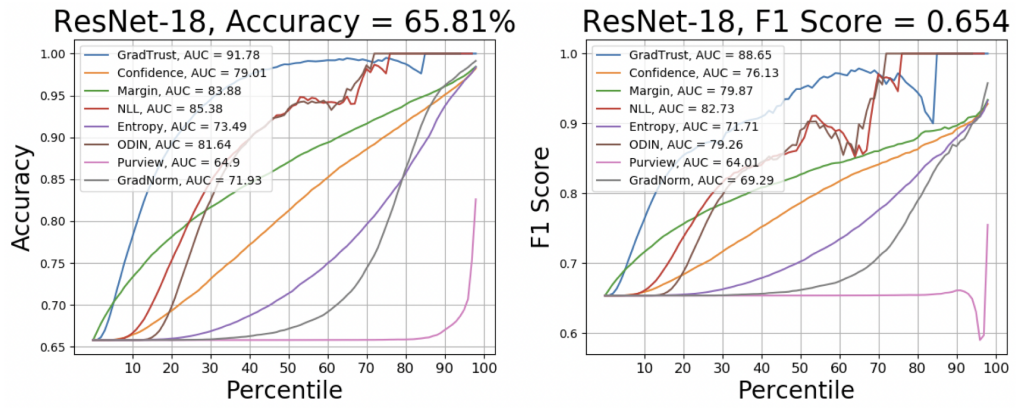
\includegraphics[width=1\linewidth]{img/lecture27/gradtrust.png}
    \caption{Figure 27.10: Example of per-dataset uncertainty evaluation using ImageNet.}
    \label{fig:gradtrust}
\end{figure}

As shown in Fig.~\ref{fig:gradtrust}, higher uncertainty typically corresponds to lower accuracy and F1 scores. Ideally, a good uncertainty estimator should rank incorrect predictions as highly uncertain. Larger AUAC and AUFC values indicate better performance because they show that the model maintains strong prediction performance even as uncertain samples are included.

This type of evaluation is particularly useful because it measures whether uncertainty estimates behave meaningfully at scale rather than only at the individual prediction level.

\subsection{Applications}

In many cases, uncertainty is evaluated indirectly through its impact on downstream applications rather than through standalone metrics. In these settings, the usefulness of uncertainty estimates is measured by how much they improve task performance.

One important example is active learning. In active learning, uncertainty estimates are used to construct acquisition functions that select informative samples for labeling. The effectiveness of uncertainty estimation can therefore be measured by how quickly model performance improves when trained on samples selected using uncertainty-based acquisition strategies.

Other applications where uncertainty estimation plays an important role include open-set recognition, where models must detect inputs from unknown classes, uncertainty visualization for model debugging, and latent space analysis for understanding model representations. Although these topics are beyond the scope of this course, they illustrate how uncertainty estimation is often evaluated based on practical usefulness rather than purely theoretical criteria.

Overall, performance evaluation for uncertainty estimation should be viewed as application-dependent. Rather than relying on a single universal metric, practitioners typically choose evaluation methods that best reflect the intended use of uncertainty estimates.

\section{Q\&A Section}

\begin{enumerate}

\item Which of the following best describes the goal of uncertainty quantification in neural networks?

\begin{enumerate}
    \item To improve training speed by reducing the number of model parameters
    \item To measure how confident a model is in its predictions
    \item To eliminate all noise in the data
    \item To replace model evaluation metrics such as accuracy
\end{enumerate}

\textbf{Solution:} \\
b) To measure how confident a model is in its predictions

\textbf{Explanation:} \\
Uncertainty quantification is used to estimate how reliable or confident a model is about its prediction. This is especially important in safety-critical tasks, where a prediction alone may not be sufficient. A model that can identify when it is uncertain is often more trustworthy than a model that always outputs confident predictions.

\vspace{2mm}

\item Suppose a model is trained to classify road signs, but at test time it encounters a completely new object that never appeared in training. Which type of uncertainty is most directly involved?

\begin{enumerate}
    \item Aleatoric uncertainty
    \item Epistemic uncertainty
    \item Deterministic uncertainty
    \item Measurement uncertainty only
\end{enumerate}

\textbf{Solution:} \\
b) Epistemic uncertainty

\textbf{Explanation:} \\
Epistemic uncertainty arises when the model lacks sufficient knowledge about the input space. If the test sample is out-of-distribution or not well represented in training data, the model may not know how to respond reliably. This type of uncertainty can often be reduced by collecting more diverse training data.

\vspace{2mm}

\item Which statement best distinguishes aleatoric uncertainty from epistemic uncertainty?

\begin{enumerate}
    \item Aleatoric uncertainty is always larger than epistemic uncertainty
    \item Aleatoric uncertainty arises from noisy or ambiguous data, while epistemic uncertainty arises from limited model knowledge
    \item Aleatoric uncertainty only applies to regression, while epistemic uncertainty only applies to classification
    \item Aleatoric uncertainty can always be removed with enough training data
\end{enumerate}

\textbf{Solution:} \\
b) Aleatoric uncertainty arises from noisy or ambiguous data, while epistemic uncertainty arises from limited model knowledge

\textbf{Explanation:} \\
Aleatoric uncertainty is associated with the data itself, such as measurement noise, occlusion, or ambiguous inputs. Epistemic uncertainty, in contrast, reflects the model's lack of knowledge and can often be reduced by improving the model or expanding the training dataset.

\vspace{2mm}

\item Why are deep ensembles considered an iterative uncertainty estimation method?

\begin{enumerate}
    \item Because the same network is trained once and evaluated once
    \item Because they iteratively modify the labels of the dataset
    \item Because they generate multiple predictions from independently trained models and combine them
    \item Because they remove uncertain samples during preprocessing
\end{enumerate}

\textbf{Solution:} \\
c) Because they generate multiple predictions from independently trained models and combine them

\textbf{Explanation:} \\
Deep ensembles estimate uncertainty by training multiple models with different initializations and aggregating their predictions. The variation across these predictions provides information about model uncertainty. Since multiple models or passes are involved, this falls under iterative uncertainty estimation.

\vspace{2mm}

\item What is the main idea behind Monte Carlo dropout?

\begin{enumerate}
    \item Use dropout only during training and disable it at test time
    \item Apply dropout during both training and inference, and average multiple stochastic predictions
    \item Replace dropout with batch normalization during inference
    \item Train many fully independent models from scratch
\end{enumerate}

\textbf{Solution:} \\
b) Apply dropout during both training and inference, and average multiple stochastic predictions

\textbf{Explanation:} \\
Monte Carlo dropout keeps dropout active during inference so that each forward pass produces a slightly different prediction. These stochastic predictions can be averaged to form a final prediction, and their variability can be used to estimate uncertainty. This gives a computationally cheaper approximation to ensemble-style uncertainty estimation.

\vspace{2mm}

\item In the decomposition
\[
U_{total} = U_{epistemic} + U_{aleatoric},
\]
which component is typically reducible with more data or better modeling?

\begin{enumerate}
    \item Aleatoric uncertainty only
    \item Epistemic uncertainty only
    \item Both are always reducible
    \item Neither is reducible
\end{enumerate}

\textbf{Solution:} \\
b) Epistemic uncertainty only

\textbf{Explanation:} \\
Epistemic uncertainty comes from incomplete model knowledge and can often be reduced by collecting more data, improving the architecture, or better exploring the parameter space. Aleatoric uncertainty is tied to the inherent ambiguity or noise in the data and is generally not removable by modeling alone.

\vspace{2mm}

\item In a segmentation task, where would aleatoric uncertainty most likely be highest?

\begin{enumerate}
    \item In regions where the model has seen many similar training examples
    \item Along object or class boundaries where labels are inherently ambiguous
    \item Only in background regions
    \item Only when the training loss is zero
\end{enumerate}

\textbf{Solution:} \\
b) Along object or class boundaries where labels are inherently ambiguous

\textbf{Explanation:} \\
Aleatoric uncertainty is typically highest where the input itself is ambiguous. In segmentation, this often occurs near class boundaries, where neighboring pixels may belong to different classes and image resolution or noise makes the correct label less certain.

\vspace{2mm}

\item Why can single-pass uncertainty estimation be attractive in practice?

\begin{enumerate}
    \item It completely removes the need for a trained model
    \item It avoids the computational cost of multiple forward passes or multiple models
    \item It guarantees better uncertainty estimates than deep ensembles
    \item It requires no assumptions about the feature space
\end{enumerate}

\textbf{Solution:} \\
b) It avoids the computational cost of multiple forward passes or multiple models

\textbf{Explanation:} \\
Single-pass methods estimate uncertainty from one forward pass, making them more efficient in time-sensitive or resource-constrained environments. Their main tradeoff is that they often rely on additional assumptions and may produce less reliable uncertainty estimates than iterative methods.

\vspace{2mm}

\item Why can difficulty-based single-pass uncertainty methods become poorly calibrated?

\begin{enumerate}
    \item Because they only work for linear models
    \item Because uncertainty is estimated in latent feature space, which may not preserve the true geometry of the input space
    \item Because they require ground-truth labels at test time
    \item Because they eliminate all outliers before inference
\end{enumerate}

\textbf{Solution:} \\
b) Because uncertainty is estimated in latent feature space, which may not preserve the true geometry of the input space

\textbf{Explanation:} \\
If the learned feature space distorts relationships between samples, then distance- or confidence-based uncertainty estimates may no longer reflect actual ambiguity in the original input space. This can lead to calibration problems, especially for outliers or underrepresented samples.

\vspace{2mm}

\item What is the purpose of imposing a Bi-Lipschitz constraint in distance-preservation methods?

\begin{enumerate}
    \item To ensure that all feature vectors collapse to the same point
    \item To preserve meaningful distances between inputs and their latent representations
    \item To eliminate epistemic uncertainty completely
    \item To convert classification into regression
\end{enumerate}

\textbf{Solution:} \\
b) To preserve meaningful distances between inputs and their latent representations

\textbf{Explanation:} \\
A Bi-Lipschitz constraint helps ensure that distances in input space are not excessively compressed or expanded in feature space. This improves the reliability of uncertainty estimates derived from latent representations because nearby samples remain nearby and distinct samples remain distinguishable.

\vspace{2mm}

\item Which of the following is a \textit{per-sample} uncertainty evaluation metric?

\begin{enumerate}
    \item Area Under the Accuracy Curve (AUAC)
    \item Open-set recognition accuracy
    \item Negative Log-Likelihood (NLL)
    \item Active learning label efficiency
\end{enumerate}

\textbf{Solution:} \\
c) Negative Log-Likelihood (NLL)

\textbf{Explanation:} \\
Per-sample metrics evaluate the quality of uncertainty for individual predictions, usually when ground-truth labels are known. NLL and Brier score are common examples. In contrast, AUAC and active learning performance are dataset- or application-level measures.

\vspace{2mm}

\item What does a lower Brier score indicate?

\begin{enumerate}
    \item Worse calibration of predicted probabilities
    \item Better agreement between predicted probabilities and true outcomes
    \item Higher computational cost
    \item Greater epistemic uncertainty
\end{enumerate}

\textbf{Solution:} \\
b) Better agreement between predicted probabilities and true outcomes

\textbf{Explanation:} \\
The Brier score measures the mean squared difference between predicted probabilities and the true labels. Lower values indicate better calibrated and more accurate probabilistic predictions, while higher values indicate larger mismatch between confidence and correctness.

\vspace{2mm}

\item In misprediction detection, what should a good uncertainty estimator do?

\begin{enumerate}
    \item Assign low uncertainty to all predictions
    \item Rank incorrect predictions as more uncertain than correct predictions
    \item Maximize entropy for every sample
    \item Produce identical uncertainty scores for the entire dataset
\end{enumerate}

\textbf{Solution:} \\
b) Rank incorrect predictions as more uncertain than correct predictions

\textbf{Explanation:} \\
A useful uncertainty estimator should help distinguish reliable predictions from unreliable ones. In dataset-level evaluation, this means that incorrect predictions should generally receive higher uncertainty scores than correct predictions. This behavior leads to stronger misprediction detection performance.

\vspace{2mm}

\item Why is uncertainty often evaluated through downstream applications such as active learning?

\begin{enumerate}
    \item Because uncertainty has no relationship to model performance
    \item Because uncertainty is only meaningful in theoretical settings
    \item Because the practical value of uncertainty is often best measured by how much it improves decision-making
    \item Because per-sample metrics are always unavailable
\end{enumerate}

\textbf{Solution:} \\
c) Because the practical value of uncertainty is often best measured by how much it improves decision-making

\textbf{Explanation:} \\
In many real-world settings, the usefulness of an uncertainty estimate is not judged only by a standalone numerical metric, but by whether it improves a downstream task. For example, in active learning, better uncertainty estimates should lead to better sample selection and faster model improvement.

\end{enumerate}

\end{document}
